% Informe independiente: cifras transcritas de la ejecucion completa suministrada.
\documentclass[11pt,a4paper]{article}
\usepackage[utf8]{inputenc}
\usepackage[T1]{fontenc}
\usepackage[spanish,es-tabla,es-nodecimaldot]{babel}
\spanishplainpercent
\usepackage{lmodern}
\usepackage[margin=2.2cm]{geometry}
\usepackage{amsmath,amssymb,graphicx,booktabs,array}
\usepackage{caption}
\usepackage{float}
\usepackage{microtype}
\usepackage[hidelinks]{hyperref}
\graphicspath{{../figuras/}}
\captionsetup{font=small,labelfont=bf}
\setlength{\parindent}{0pt}
\setlength{\parskip}{6pt}
\setlength{\emergencystretch}{1em}
\newcommand{\archivo}[1]{\texttt{#1}}
\newcommand{\cientifico}[2]{\ensuremath{#1\times10^{#2}}}
\hypersetup{pdftitle={Reconocimiento facial mediante valores propios},
  pdfauthor={Génesis Conejo Montero; Aldo Alessandro Bagliano Gómez; Joel David Barboza Picado}}

\begin{document}

% La portada reproduce los datos proporcionados; no se agrega una fecha ausente.
\hypersetup{pageanchor=false}
\begin{titlepage}
\centering
\vspace*{0.4cm}
{\large Instituto Tecnológico de Costa Rica\par}
\vspace{1.5cm}
{\large Ingeniería en Computadores\par}
\vspace{1.5cm}
{\large CE-1111 -- Análisis Numérico para Ingeniería\par}
\vspace{0.3cm}
{\large Portafolio Computacional -- Bloque 3\par}
\vspace{0.9cm}
{\Large\bfseries Parte III\par}
\vspace{0.25cm}
{\Large\bfseries Aplicación -- Reconocimiento facial\par}
{\Large\bfseries mediante valores propios\par}
\vspace{1.5cm}
{\large Profesor:\par}
\vspace{0.3cm}
{\large Juan Pablo Soto Quirós\par}
\vfill
{\large Integrantes:\par}
\vspace{0.4cm}
\begin{tabular}{l@{\quad|\quad}l}
Génesis Conejo Montero & 2023083122\\[5pt]
Aldo Alessandro Bagliano Gómez & 2020018456\\[5pt]
Joel David Barboza Picado & 2023218734
\end{tabular}
\vspace*{1.7cm}
\end{titlepage}
\hypersetup{pageanchor=true}

% Pasos 1 a 4: preparar datos sin utilizar las fotografias de prueba.
\section{Objetivo y preparación de los datos}
El objetivo fue identificar la persona a la que pertenece cada fotografía de prueba
entre las 40 identidades conocidas de la base AT\&T. Se aplicó el procedimiento de
los Pasos 1 al 8 de la guía del curso, con los requisitos de la Parte III del
enunciado. La evaluación corresponde a identificación entre
personas conocidas; no mide la detección ni el rechazo de personas desconocidas.

\subsection{Organización y separación}
Se utilizaron las carpetas \archivo{s1} a \archivo{s40}. Para cada persona,
\archivo{1.png} a \archivo{9.png} se destinaron a entrenamiento y únicamente
\archivo{10.png} se reservó para prueba. Las columnas se ordenaron primero por
número de persona y después por número de fotografía, conservando etiquetas y rutas
en ese mismo orden. Así, \archivo{s2} precede a \archivo{s10}.

\begin{table}[h]
\centering
\caption{Separación fija de las fotografías de las 40 personas.}
\begin{tabular}{lccc}
\toprule
Conjunto & Archivos por persona & Por persona & Total\\
\midrule
Entrenamiento & \archivo{1.png} a \archivo{9.png} & 9 & 360\\
Prueba & \archivo{10.png} & 1 & 40\\
\bottomrule
\end{tabular}
\end{table}

\subsection{Normalización, vectorización y centrado}
Se conservó la resolución original de 56 filas por 46 columnas, en escala de grises.
Las intensidades se convirtieron a punto flotante y se dividieron entre 255.
Cada imagen se vectorizó por columnas, recorriendo primero los 56 píxeles de la
primera columna y luego los de las siguientes hasta obtener $f_i\in\mathbb{R}^{2576}$.
La matriz de entrenamiento fue
\begin{equation}
S=[f_1\;f_2\;\cdots\;f_{360}]\in\mathbb{R}^{2576\times360}.
\end{equation}
El rostro promedio y los datos centrados se calcularon exclusivamente con esas
360 fotografías mediante las expresiones
\begin{equation}
\bar f=\frac{1}{360}\sum_{i=1}^{360}f_i,
\qquad a_i=f_i-\bar f,
\qquad A=[a_1\;\cdots\;a_{360}]\in\mathbb{R}^{2576\times360}.
\end{equation}
La normalización produjo intensidades entre 0.01960784 y 0.91764706, dentro de
$[0,1]$. La reconstrucción de la primera imagen a partir de su vector tuvo error
máximo cero. El promedio absoluto máximo de las filas de $A$ fue
\cientifico{1.480297}{-16}, compatible con el centrado en precisión de máquina.
Las fotografías de prueba no participaron en estos cálculos ni en la selección
de las caras base.

\clearpage
% Pasos 5 a 8: construir la base, proyectar e identificar con el modelo fijo.
\section{Construcción del modelo e identificación}
La matriz exigida por la guía se construyó como
\begin{equation}
G=AA^{\mathsf T}\in\mathbb{R}^{2576\times2576}.
\end{equation}
Los pares propios se calcularon con \archivo{metodo\_jacobi}, importado de
\archivo{parte1.py}, usando $\mathrm{iterMax}=10^6$ y
$\mathrm{tol}=10^{-5}$. No se sustituyó $G$ por $A^{\mathsf T}A$, no se redujo la
resolución y no se emplearon funciones de biblioteca que resolvieran directamente
los valores o vectores propios.

Los valores propios se ordenaron de mayor a menor, aplicando exactamente la misma
permutación a las columnas de vectores propios. Se retuvieron los pares que
satisfacen
\begin{equation}
\lambda_j>10^{-10}\lambda_1,
\qquad \lambda_1\geq\lambda_2\geq\cdots\geq\lambda_r>0,
\end{equation}
donde $r$ es el número de valores retenidos. Los vectores normalizados asociados
constituyen las caras base. Se seleccionó el menor entero $k$ tal que
\begin{equation}
\frac{\sum_{j=1}^{k}\lambda_j}{\sum_{j=1}^{r}\lambda_j}\geq0.95.
\end{equation}
Con las primeras $k$ caras base se formaron
\begin{equation}
U_k=[u_1\;\cdots\;u_k],\qquad X=U_k^{\mathsf T}A.
\end{equation}
La columna $i$ de $X$ contiene las coordenadas de la fotografía de entrenamiento
$i$ y conserva su etiqueta $y_i$. Para cada consulta se aplicaron la misma
normalización y vectorización; luego se calculó
\begin{equation}
x=U_k^{\mathsf T}(f-\bar f),\qquad
d_i=\lVert x-X_{:,i}\rVert_2,\quad i=1,\ldots,360.
\end{equation}
La identidad predicha fue $y_{i^*}$, con $i^*=\arg\min_i d_i$. En empate exacto
se eligió la primera fotografía según el orden numérico establecido. La
comparación se hizo contra las 360 fotografías de entrenamiento, no contra otras
consultas ni contra promedios individuales por persona.

El promedio, $U_k$, $X$ y $k$ se mantuvieron fijos durante las 40 pruebas. No se
reentrenó el modelo ni se ajustó $k$ después de observar los aciertos o las
confusiones. Las cifras y figuras de este informe proceden de la ejecución
completa suministrada; no son resultados ilustrativos de la guía.

\clearpage
% Comparacion real y diagnosticos independientes del indicador de convergencia.
\section{Selección del método y calidad numérica}
\subsection{Comparación de QR y Jacobi}
La comparación utilizó la matriz tridiagonal de $200\times200$ de la Parte II,
con diagonal principal 4 y diagonales adyacentes $-1$, usando
$\mathrm{iterMax}=10000$ y $\mathrm{tol}=10^{-8}$.
La Tabla~\ref{tab:comparacion} resume las funciones existentes de \archivo{parte1.py}.

\begin{table}[h]
\centering
\caption{Comparación real sobre la matriz de $200\times200$.}
\label{tab:comparacion}
\begin{tabular}{lcc}
\toprule
Medida & QR & Jacobi\\
\midrule
Error final $er_k$ & \cientifico{1.1596}{-6} & \cientifico{2.1173}{-9}\\
Iteraciones / barridos & 10000 & 11\\
Tiempo (s) & 68.2118 & 2.5781\\
Indicador $\mathrm{conv}$ & 0 & 1\\
Residuo máximo & \cientifico{4.7931}{-3} & \cientifico{4.9991}{-11}\\
$\lVert V^{\mathsf T}V-I\rVert_F$ & \cientifico{4.1331}{-13} & \cientifico{5.6763}{-14}\\
\bottomrule
\end{tabular}
\end{table}

Se eligió Jacobi porque alcanzó la tolerancia, obtuvo un residuo máximo mucho
menor y empleó menos tiempo en esta ejecución. Ambos métodos conservaron bien la
ortogonalidad; por tanto, esta medida por sí sola no explica la elección. QR
agotó las 10000 iteraciones sin cumplir el umbral de parada. Una iteración QR
realiza una factorización y actualización de la matriz, mientras que un barrido
Jacobi recorre los pares de índices y aplica las rotaciones necesarias. Sus
conteos no representan unidades de trabajo equivalentes. Estos resultados no
demuestran que Jacobi siempre supere a QR para otras matrices o implementaciones.

\subsection{Comprobaciones sobre la matriz G}
\begin{table}[h]
\centering
\caption{Resultado de Jacobi y calidad de los 2576 pares propios de $G$.}
\label{tab:calidad}
\begin{tabular}{lc}
\toprule
Medida & Valor\\
\midrule
$\mathrm{iterMax}$; $\mathrm{tol}$ & $10^6$; $10^{-5}$\\
Barridos; $\mathrm{conv}$ & 9; 1\\
Error final $er_k$ & \cientifico{2.463650}{-8}\\
Tiempo & 2981.40 s (49.69 min)\\
Residuo máximo & \cientifico{4.025927}{-9}\\
Residuo máximo / $\lVert G\rVert_F$ & \cientifico{7.237988}{-13}\\
$\lVert V^{\mathsf T}V-I\rVert_F$ & \cientifico{6.465629}{-13}\\
$\max_j|\lVert v_j\rVert_2-1|$ & \cientifico{2.220446}{-16}\\
\bottomrule
\end{tabular}
\end{table}

El error de parada fue $er_k=\lVert\lambda^{(k)}-\lambda^{(k-1)}\rVert_2$, con
los valores aproximados ordenados. Mide su cambio entre barridos, no el residuo
de cada par. Se verificaron adicionalmente
$\lVert Gv_j-\lambda_jv_j\rVert_2$, la ortogonalidad y las normas de todos los
vectores. Sus errores pequeños respaldan la calidad numérica; no se tomó
$\mathrm{conv}=1$ como garantía suficiente. El tiempo reportado corresponde al
método sobre $G$, sin incluir la comparación inicial ni la presentación de figuras.

\clearpage
% Figura original del programa y justificacion del minimo k.
\section{Rostro promedio y selección de componentes}
\begin{figure}[H]
\centering
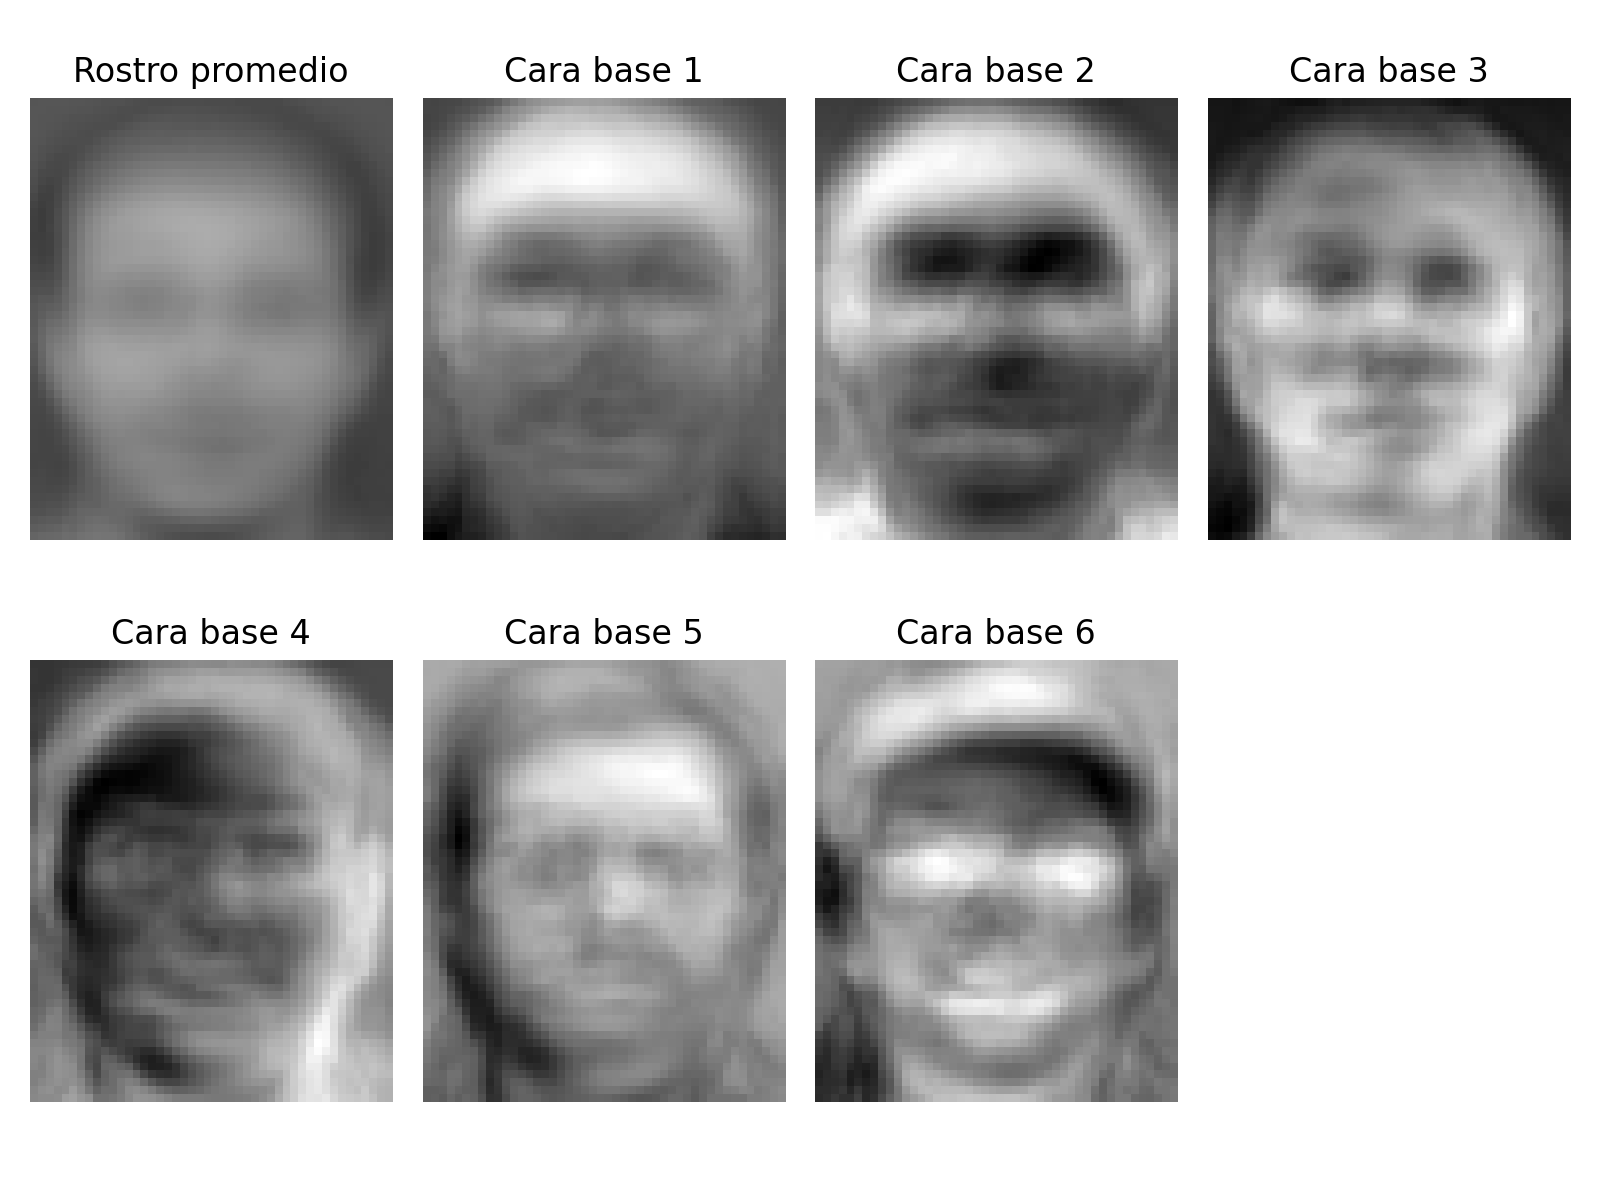
\includegraphics[width=0.92\textwidth]{caras_base.png}
\caption{Rostro promedio y primeras seis caras base de esta ejecución, calculados
exclusivamente con las 360 fotografías de entrenamiento.}
\label{fig:caras}
\end{figure}

El promedio se ve difuso porque combina las intensidades de diferentes rostros.
Las caras base representan patrones de variación de las imágenes centradas, no
necesariamente personas concretas. Las regiones claras y oscuras corresponden a
las entradas del vector visualizado con una escala ajustada. Invertir el signo de
un vector propio no cambia su validez ni las distancias entre proyecciones si se
usa el mismo signo en entrenamiento y prueba.

\begin{table}[h]
\centering
\caption{Componentes retenidas y dimensiones del espacio reducido.}
\begin{tabular}{lc}
\toprule
Resultado & Valor\\
\midrule
Valores propios retenidos $r$ & 359\\
Caras base seleccionadas $k$ & 129\\
Variación con $k$ & 95.00743277\,\%\\
Variación con $k-1$ & 94.94904164\,\%\\
Dimensiones de $U_k$ & $2576\times129$\\
Dimensiones de $X$ & $129\times360$\\
\bottomrule
\end{tabular}
\end{table}

Como 128 componentes no alcanzan el 95\,\% y 129 sí, $k=129$ es el mínimo
admisible. Se calculó a partir de los valores propios retenidos, sin fijarlo con
una cifra de referencia. El valor $r=359$ es coherente con 360 columnas centradas,
cuyo rango no puede superar 359. Cada fotografía pasa de 2576 intensidades a
129 coordenadas para la comparación; la reducción se hace después de leer la
imagen completa, sin cambiar su resolución.

\clearpage
% Las cuarenta filas se transcriben explicitamente de la salida de terminal.
\section{Predicciones y exactitud}
La Tabla~\ref{tab:predicciones} incluye las 40 consultas reservadas, en el mismo
orden de la ejecución. Hubo 38 identificaciones correctas y dos confusiones, por lo
que la exactitud fue
\begin{equation}
\mathrm{Exactitud}=100\frac{38}{40}=95\,\%.
\end{equation}
Conservar el 95\,\% de variación no garantiza un 95\,\% de exactitud. La primera
medida describe información del entrenamiento; la segunda cuenta aciertos en
las consultas. Su coincidencia aproximada aquí no establece una garantía.

\begin{table}[h]
\centering
\caption{Predicciones completas de las fotografías de prueba.}
\label{tab:predicciones}
\small
\setlength{\tabcolsep}{12pt}
\renewcommand{\arraystretch}{1.02}
\begin{tabular}{lccc}
\toprule
Archivo & Persona real & Persona predicha & ¿Acertó?\\
\midrule
\archivo{s1/10.png} & 1 & 1 & Sí\\
\archivo{s2/10.png} & 2 & 2 & Sí\\
\archivo{s3/10.png} & 3 & 3 & Sí\\
\archivo{s4/10.png} & 4 & 4 & Sí\\
\archivo{s5/10.png} & 5 & 40 & No\\
\archivo{s6/10.png} & 6 & 6 & Sí\\
\archivo{s7/10.png} & 7 & 7 & Sí\\
\archivo{s8/10.png} & 8 & 8 & Sí\\
\archivo{s9/10.png} & 9 & 9 & Sí\\
\archivo{s10/10.png} & 10 & 38 & No\\
\archivo{s11/10.png} & 11 & 11 & Sí\\
\archivo{s12/10.png} & 12 & 12 & Sí\\
\archivo{s13/10.png} & 13 & 13 & Sí\\
\archivo{s14/10.png} & 14 & 14 & Sí\\
\archivo{s15/10.png} & 15 & 15 & Sí\\
\archivo{s16/10.png} & 16 & 16 & Sí\\
\archivo{s17/10.png} & 17 & 17 & Sí\\
\archivo{s18/10.png} & 18 & 18 & Sí\\
\archivo{s19/10.png} & 19 & 19 & Sí\\
\archivo{s20/10.png} & 20 & 20 & Sí\\
\archivo{s21/10.png} & 21 & 21 & Sí\\
\archivo{s22/10.png} & 22 & 22 & Sí\\
\archivo{s23/10.png} & 23 & 23 & Sí\\
\archivo{s24/10.png} & 24 & 24 & Sí\\
\archivo{s25/10.png} & 25 & 25 & Sí\\
\archivo{s26/10.png} & 26 & 26 & Sí\\
\archivo{s27/10.png} & 27 & 27 & Sí\\
\archivo{s28/10.png} & 28 & 28 & Sí\\
\archivo{s29/10.png} & 29 & 29 & Sí\\
\archivo{s30/10.png} & 30 & 30 & Sí\\
\archivo{s31/10.png} & 31 & 31 & Sí\\
\archivo{s32/10.png} & 32 & 32 & Sí\\
\archivo{s33/10.png} & 33 & 33 & Sí\\
\archivo{s34/10.png} & 34 & 34 & Sí\\
\archivo{s35/10.png} & 35 & 35 & Sí\\
\archivo{s36/10.png} & 36 & 36 & Sí\\
\archivo{s37/10.png} & 37 & 37 & Sí\\
\archivo{s38/10.png} & 38 & 38 & Sí\\
\archivo{s39/10.png} & 39 & 39 & Sí\\
\archivo{s40/10.png} & 40 & 40 & Sí\\
\bottomrule
\end{tabular}
\end{table}

\clearpage
% Analisis de hechos observados, hipotesis y limitaciones de la evaluacion.
\section{Análisis de las confusiones y de la reducción de dimensión}
Las dos confusiones corresponden a las parejas señaladas en rojo en la
Figura~\ref{fig:parejas1}. Para \archivo{s5/10.png}, el vecino fue
\archivo{s40/5.png}, con distancia 4.201565. Ambas fotografías presentan una
vista casi frontal, una frente clara y regiones más oscuras alrededor de los
ojos y el cabello. La consulta muestra una sonrisa más marcada, mientras que el
vecino tiene una expresión distinta; también difieren los rasgos y el contorno.
El hecho comprobado es que, con las coordenadas seleccionadas, ese vecino de la
persona 40 quedó más cerca que las fotografías de entrenamiento de la persona 5.

Para \archivo{s10/10.png}, el vecino fue \archivo{s38/4.png}, con distancia
6.609280. Se observan cabello oscuro, una región clara en la frente y sombras
alrededor de los ojos en ambas imágenes. Son visibles diferencias en la boca,
la expresión y el contorno facial. La predicción confirma una proximidad mayor
a la persona 38 en el espacio reducido; no demuestra que las dos fotografías
representen la misma identidad.

Las variaciones de iluminación, postura o expresión y la información descartada
son explicaciones posibles de estos errores, no causas demostradas por las 40
pruebas. Las semejanzas de intensidad pueden influir en una distancia euclidiana
sin equivaler a una coincidencia de identidad. Para atribuir cada confusión a un
factor particular harían falta experimentos adicionales con ese factor controlado.

Los vectores propios proporcionan direcciones ortogonales del espacio de imágenes
centradas; los valores propios cuantifican la variación del entrenamiento en
esas direcciones. Al seleccionar las primeras 129, se conserva la mayor parte
de esa variación con muchas menos coordenadas. La parte descartada, aproximadamente
4.9926\,\% de la variación retenida, puede contener diferencias útiles para
distinguir personas. A su vez, parte de la variación conservada puede corresponder
a iluminación o expresión, de modo que el umbral no optimiza directamente la
separación entre identidades.

La identificación por proximidad produjo 38 aciertos y dos errores bajo la
separación establecida, con pares propios de buena calidad numérica. Los
residuos pequeños respaldan el cálculo espectral, pero no garantizan la
clasificación correcta de cada rostro. El costo principal fue el cálculo de
los pares propios de $G$, que requirió 49.69 minutos en esta ejecución.

Se evaluó solamente una fotografía por identidad conocida. Por ello, el 95\,\%
describe estas 40 consultas y no mide el rendimiento ante todas las condiciones
de captura, otras divisiones de datos o personas ajenas a la base. El modelo
siempre asigna una de las 40 etiquetas; no dispone de un criterio de rechazo
de desconocidos.

\clearpage
% Las cuatro figuras originales contienen diez parejas cada una, sin regenerarlas.
\section{Fotografías de prueba y vecinos de entrenamiento}
Cada figura presenta diez consultas y sus vecinos, leídos de los archivos
originales guardados por el programa. Las etiquetas rojas marcan las dos
identificaciones incorrectas; las demás parejas acertaron la identidad.
\begin{figure}[H]
\centering
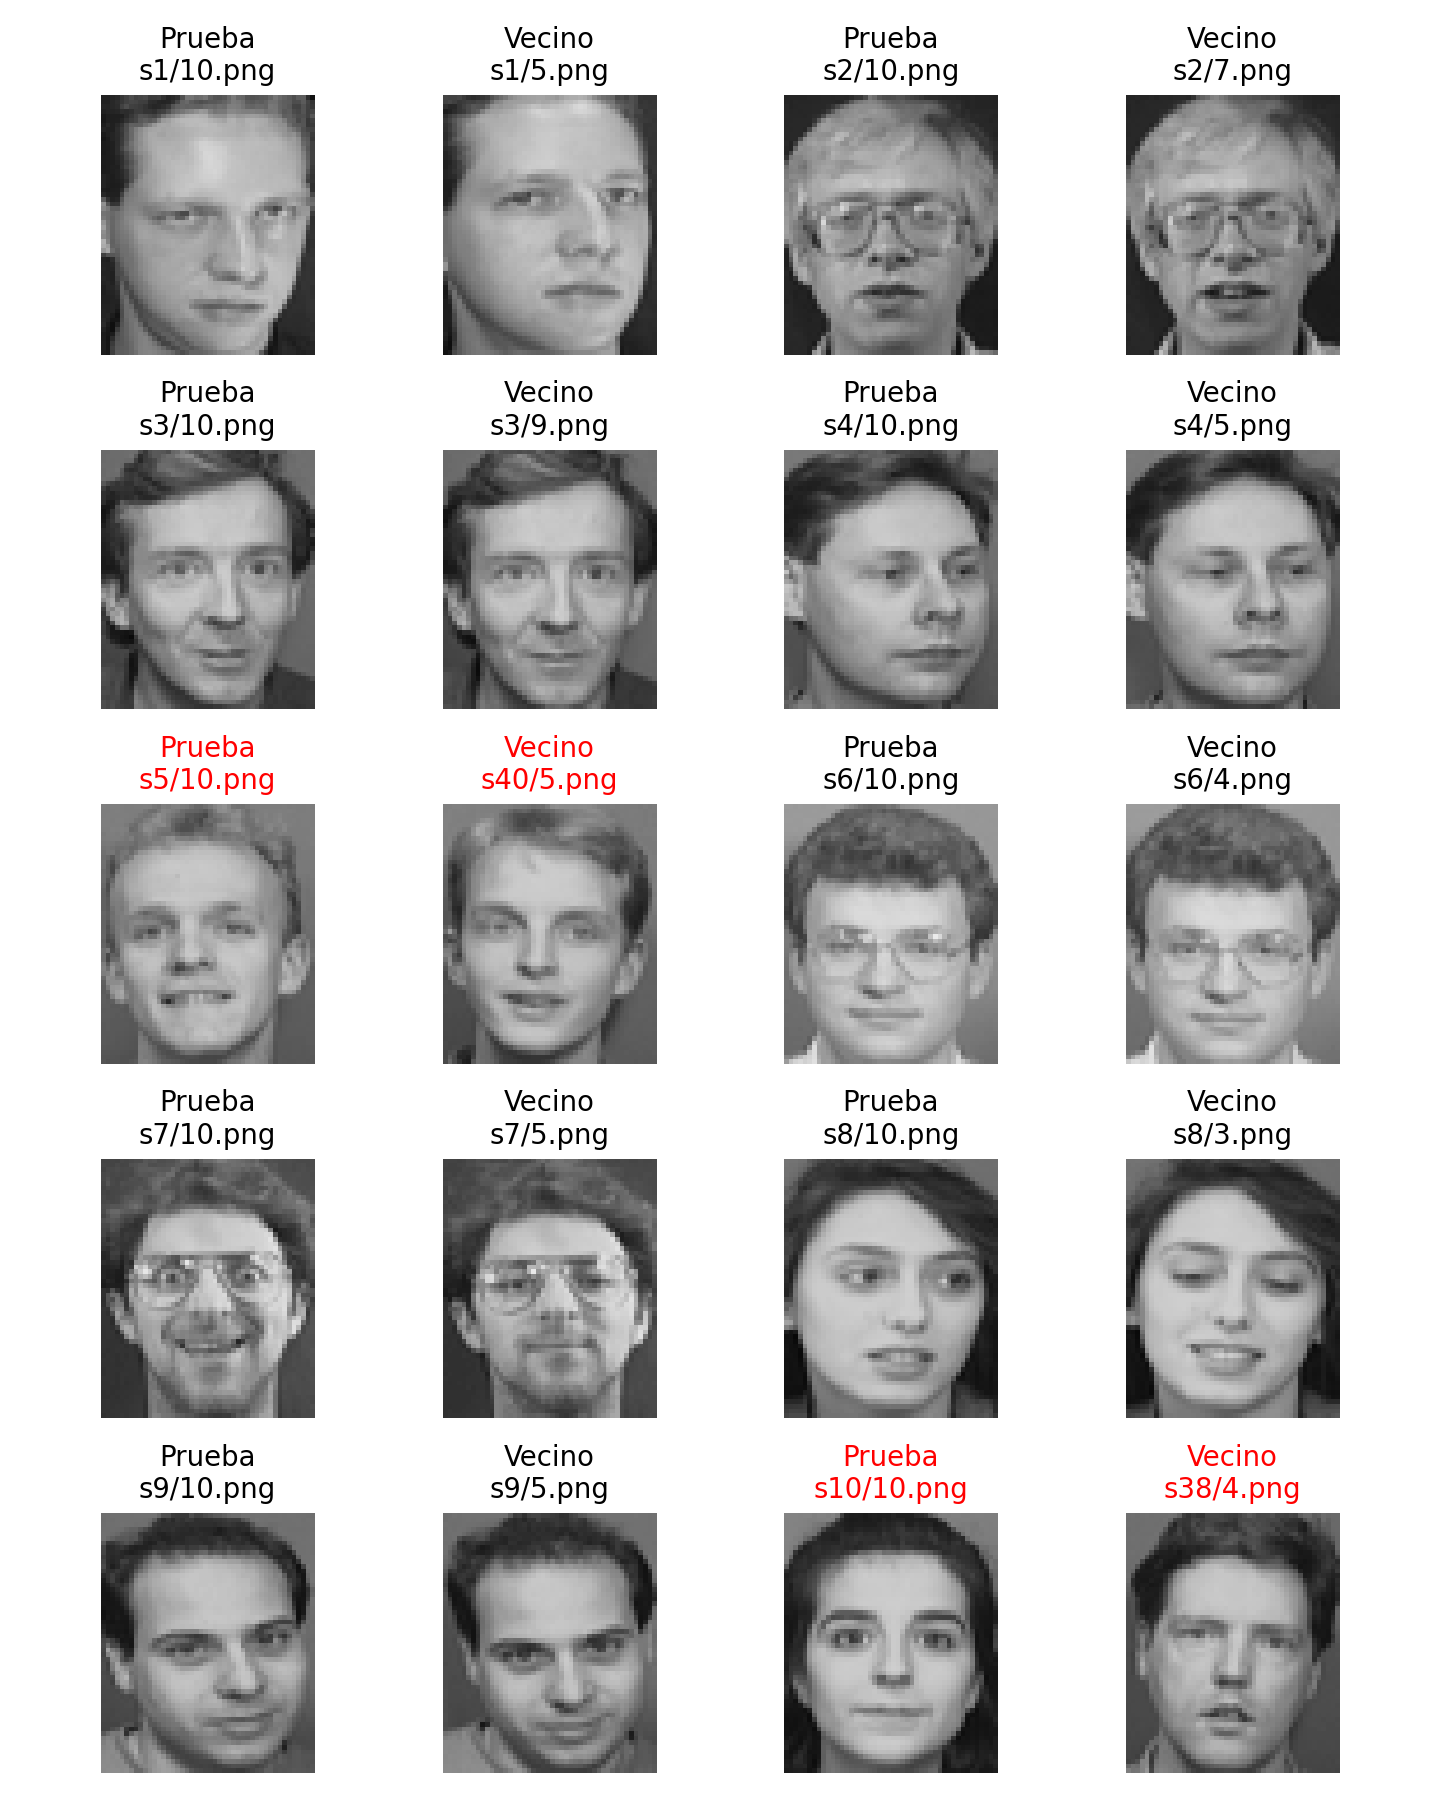
\includegraphics[width=\textwidth,height=20cm,keepaspectratio]{parejas_1.png}
\caption{Personas 1 a 10: fotografía de prueba y fotografía de entrenamiento más
cercana. Las confusiones son $5\to40$ y $10\to38$.}
\label{fig:parejas1}
\end{figure}

\clearpage
\subsection*{Personas 11 a 20}
\begin{figure}[H]
\centering
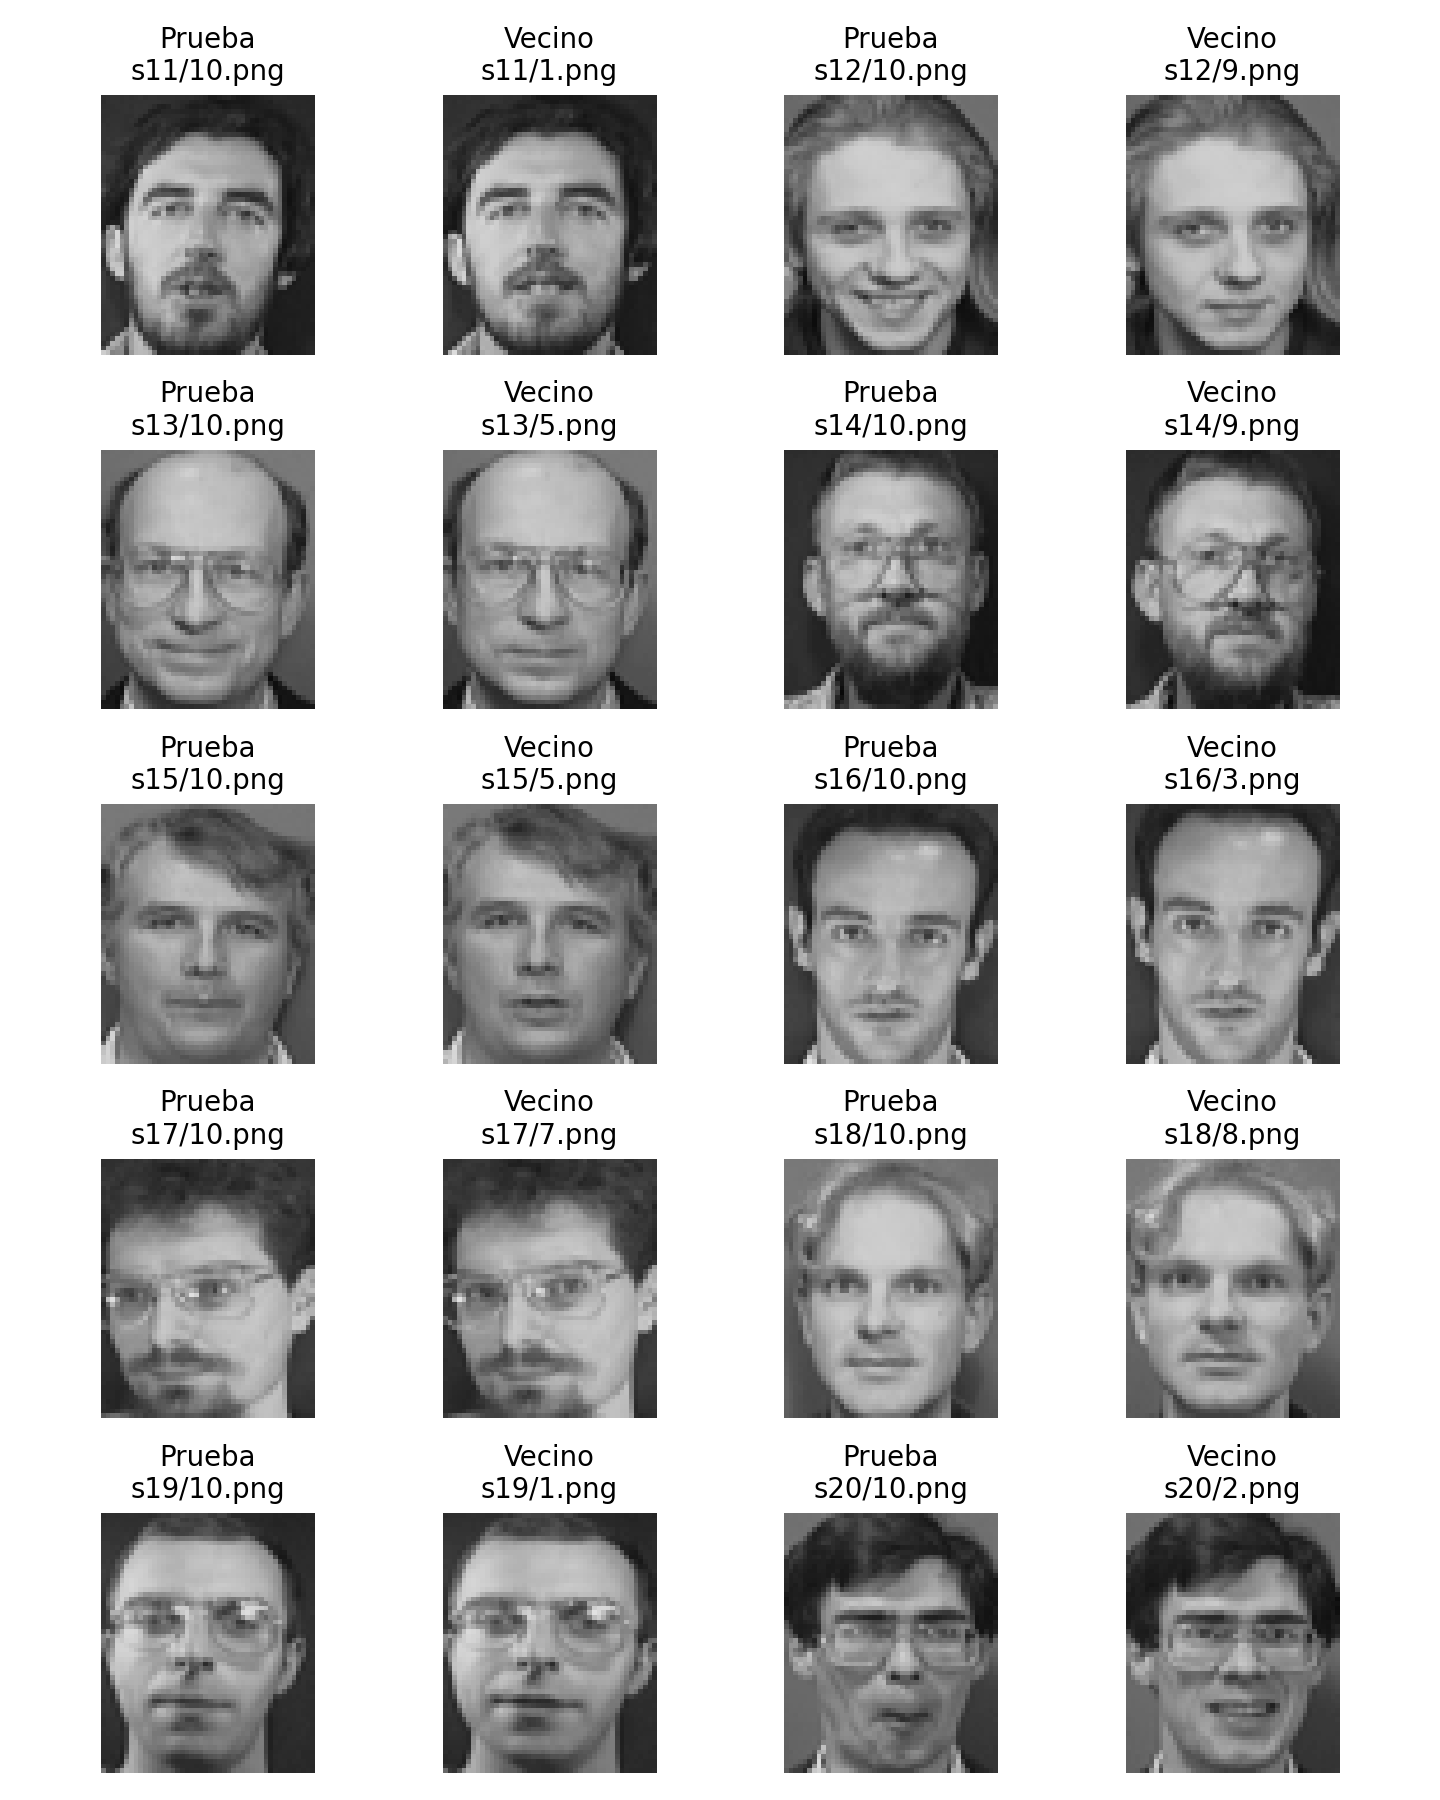
\includegraphics[width=\textwidth,height=20cm,keepaspectratio]{parejas_2.png}
\caption{Personas 11 a 20: diez parejas con identificación correcta. Las rutas
distinguen la consulta \archivo{10.png} de su vecino de entrenamiento.}
\end{figure}

\clearpage
\subsection*{Personas 21 a 30}
\begin{figure}[H]
\centering
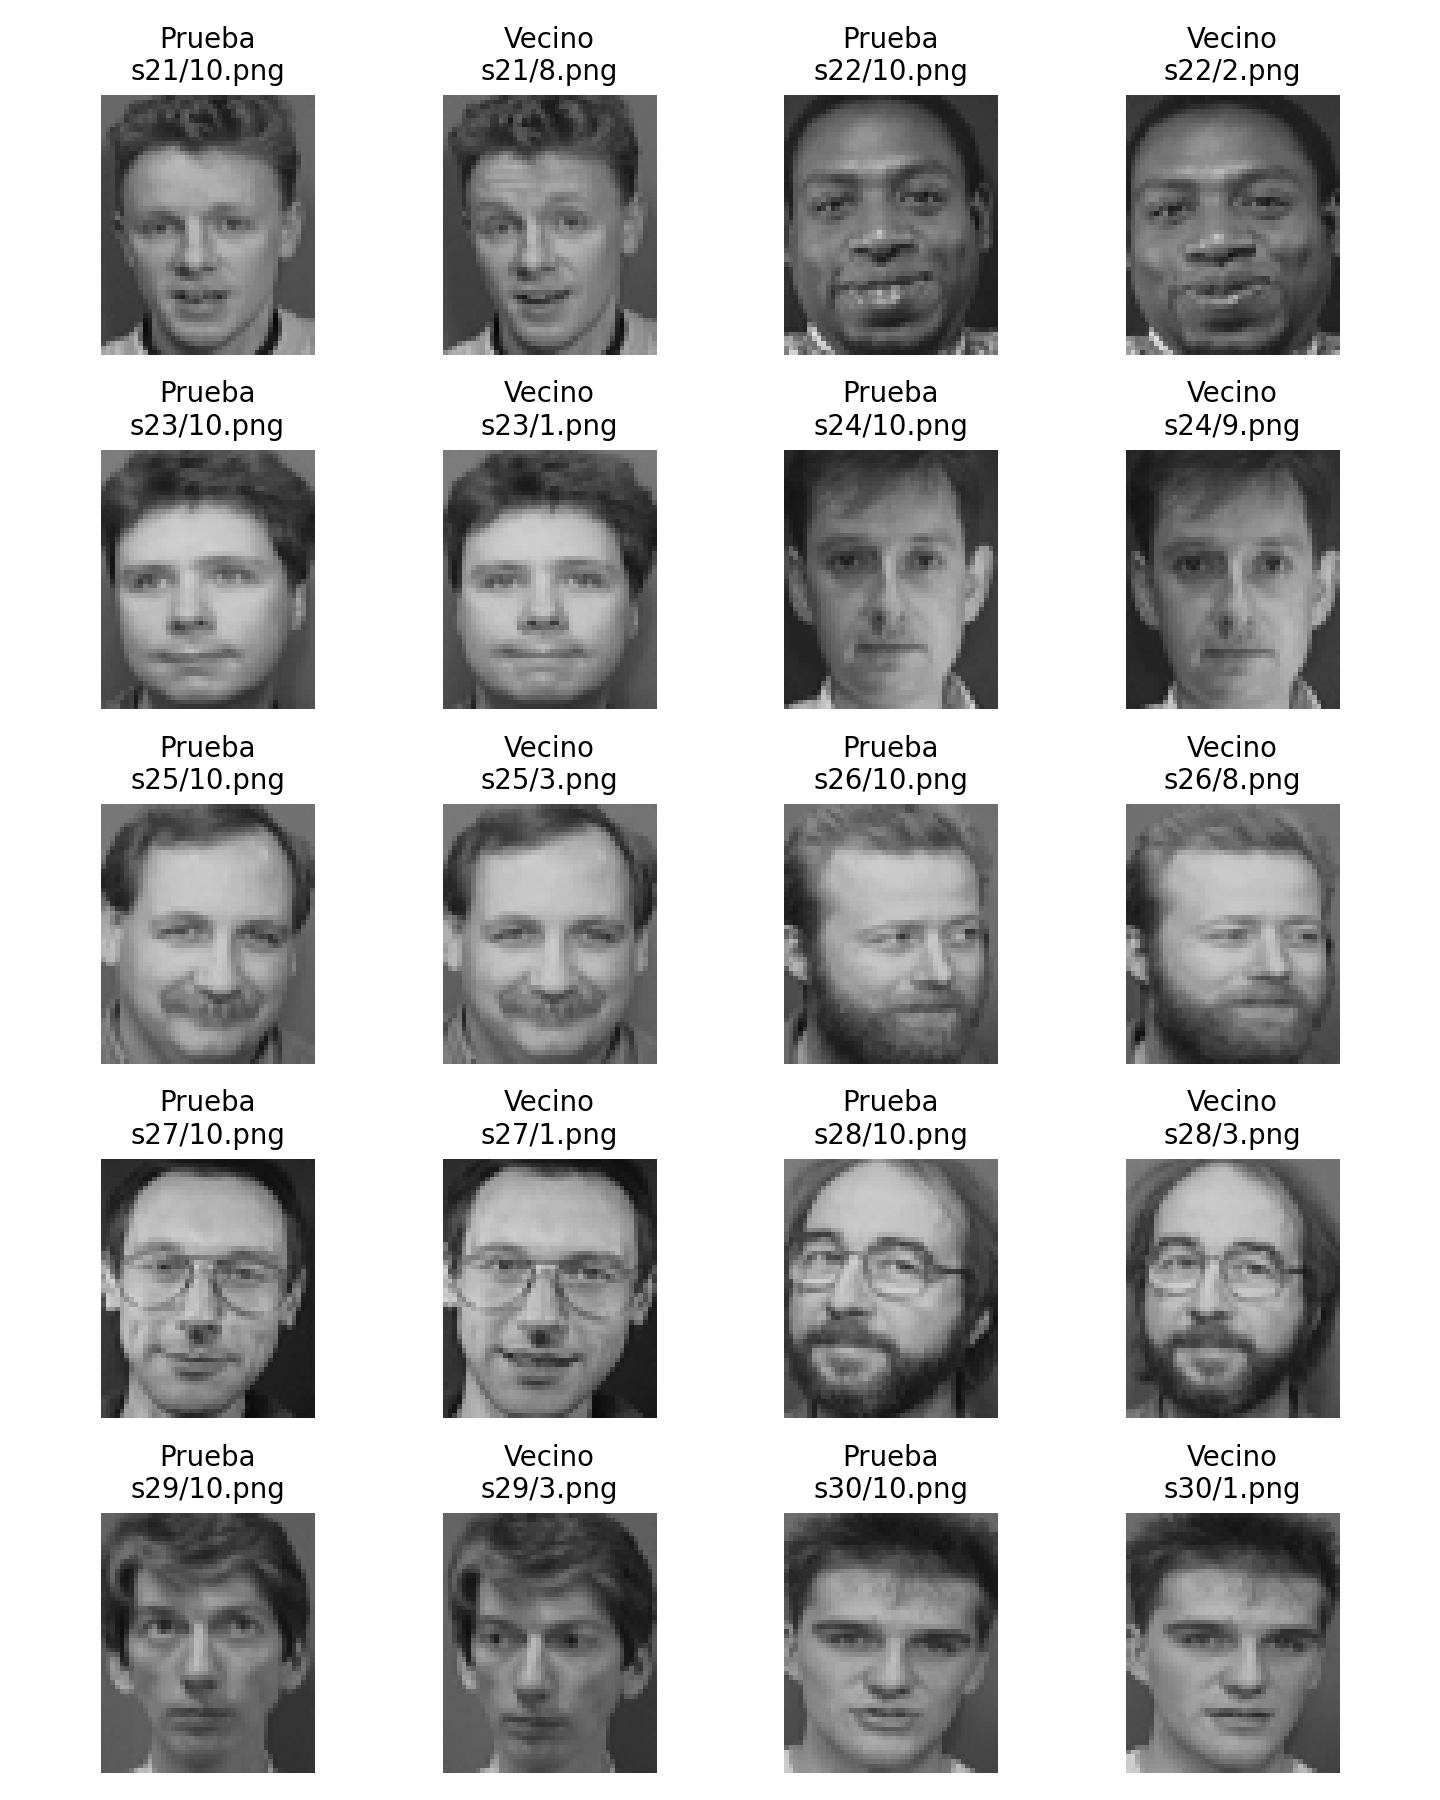
\includegraphics[width=\textwidth,height=20cm,keepaspectratio]{parejas_3.png}
\caption{Personas 21 a 30: diez parejas con identificación correcta, conservando
el mismo modelo, promedio y número de componentes.}
\end{figure}

\clearpage
\subsection*{Personas 31 a 40}
\begin{figure}[H]
\centering
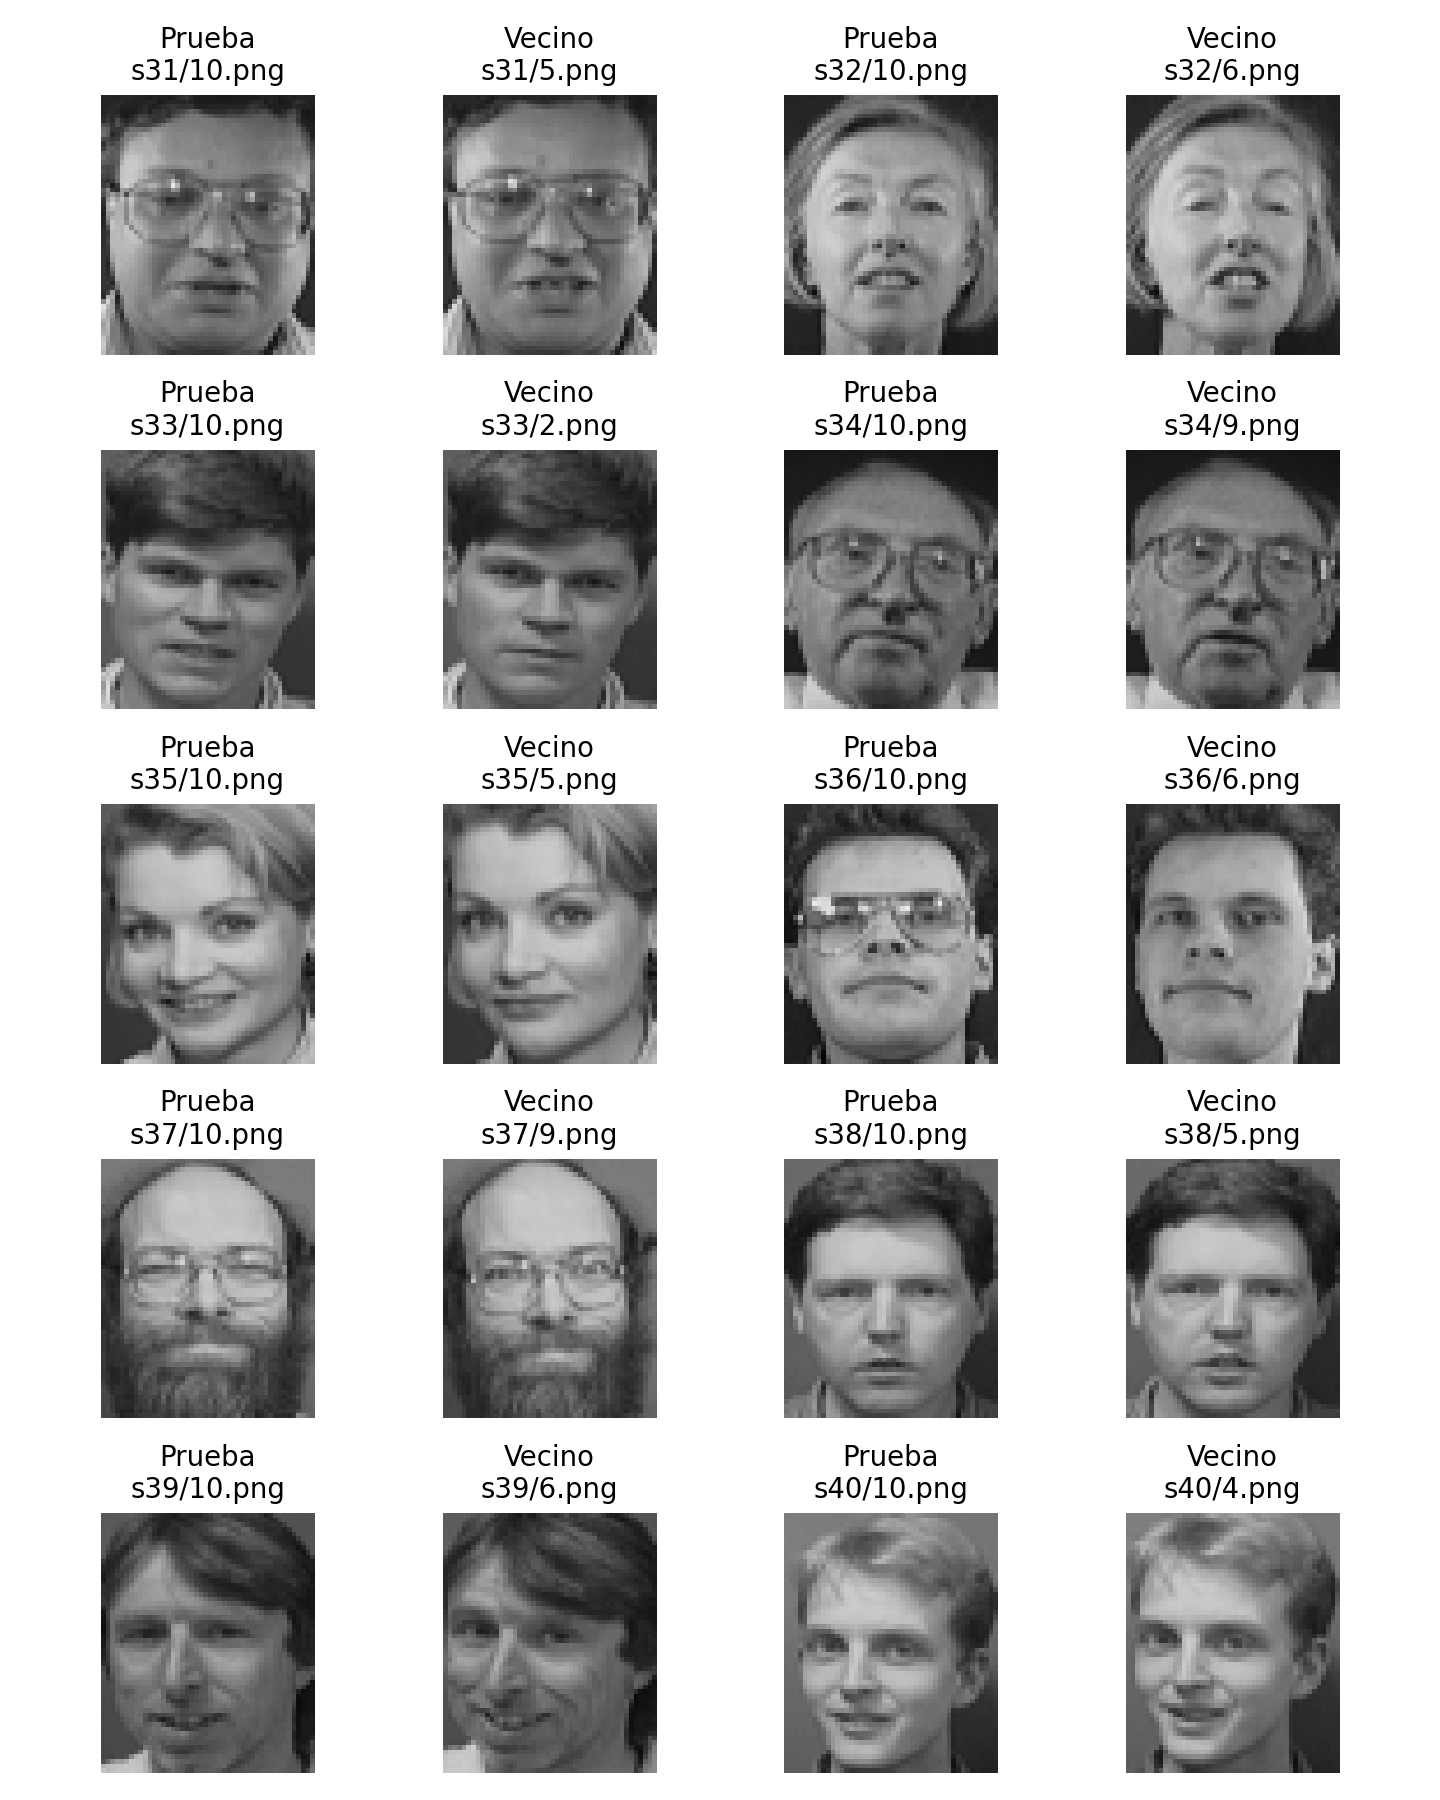
\includegraphics[width=\textwidth,height=20cm,keepaspectratio]{parejas_4.png}
\caption{Personas 31 a 40: diez parejas con identificación correcta. Esta figura
completa las 40 consultas de la evaluación.}
\end{figure}

\end{document}
